\documentclass[a4paper]{article}
\usepackage{graphicx}
\usepackage[a4paper, total={6in, 8in}]{geometry}
\pagestyle{headings}
\begin{document}

\section{Report}
\subsection{Unoptimized}

\begin{figure}[h]

\centering
\includegraphics[scale=0.75]{newest_output.png}
 \caption{Call Graph of old one }
\end{figure}

this takes a lot of time because of a long unnessessary for loop in DrawSolidCircle function in render.cpp
 after optimising the debug mode the call graph looks like this.
 \\
\\
\\
\subsection{Debug}

\begin{figure}[h]

\centering
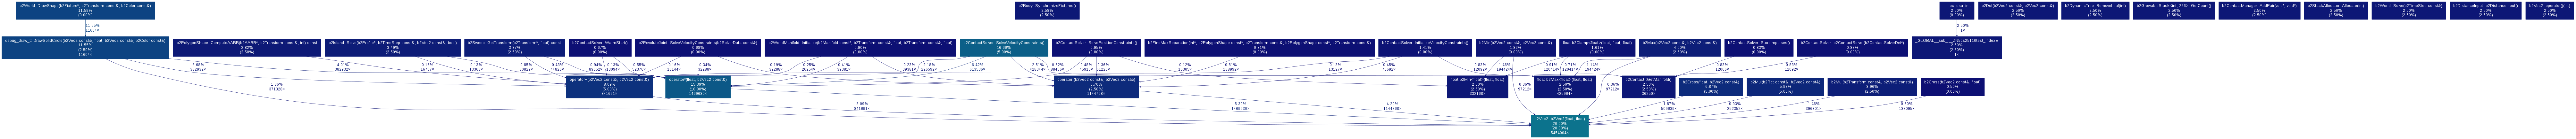
\includegraphics[width=10cm, height=6cm]{debugVersion.png}
\caption{Call Graph of Debug mode }
\end{figure}


The top 5 functions 

\begin{enumerate}
  \item b2Vec2::b2Vec2(float, float).
  \item operator*(float, b2Vec2 const\&)
  \item operator+(b2Vec2 const\&, b2Vec2 const\&)
  \item b2Mul(b2Rot const\&, b2Vec2 const\&)
  \item b2Cross(float, b2Vec2 const\&)

\end{enumerate}


\subsection{Release}

 
\begin{figure}[h]

\centering
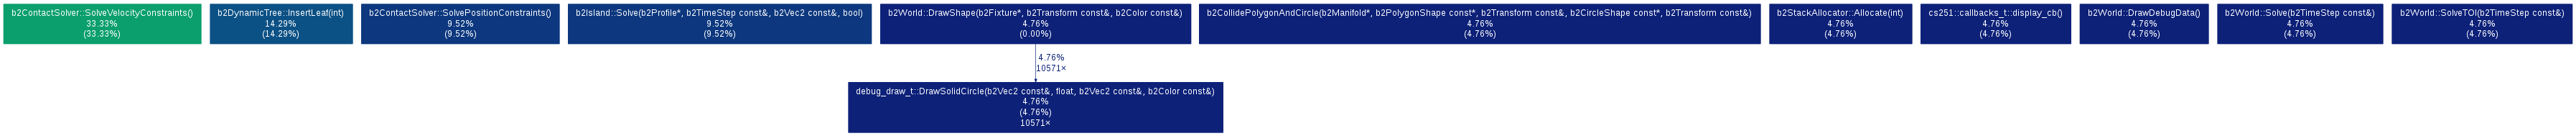
\includegraphics[width=15cm, height=3cm]{releaseVersion.png}
\caption{Call Graph of Release mode }
\end{figure}

The top 5 functions 

\begin{enumerate}
\item b2ContactSolver::SolveVelocityConstraints()
\item b2DynamicTree::InsertLeaf(int)
\item b2ContactSolver::SolvePositionConstraints()
\item b2Island::Solve(b2Profile*, b2TimeStep const\&, b2Vec2 const\&, bool)
\item  debug\_draw\_t::DrawSolidCircle(b2Vec2 const\&, float, b2Vec2 const\&, b2Color const\&)
 
\end{enumerate}

\end{document}	